\chapter{Netio3}
\label{chap:netio3}

Netio3 \cite{netio3-docs} is a transport-agnostic networking library originally created for the Phase-2 \acs{FELIX} system, offering both TCP and \acs{RDMA} communication pathways.  It is organized into two modules: the \texttt{netio3-backend} and \texttt{the netio3-frontend}.  The backend is responsible for raw data transmission and reception over the network and does not contain any \acs{FELIX}-specific logic, making it reusable in other projects. The frontend builds on this by providing buffered I/O for efficient data coalescence, a publish/subscribe API and data formatting.  Under the hood, TCP transport is implemented by the \acs{ATLAS} \acs{T-DAQ} asyncmsg library, while \acs{RDMA} operations use the \texttt{libfabric} \cite{libfabric} library.  Both transports follow a connection-oriented, message-based paradigm.

\section{Netio3 backend}

Both the asyncmsg and the \texttt{libfabric} backend use an event-driven model in the form of an event loop. Events can be callbacks from the underlying network library notifying the application about new connections, incoming data or user defined callbacks added through signals and timers. The event loop is single threaded, thus guaranteeing that all events are executed sequentially. Each event is associated with a callback that contains the user code that is executed when the event is triggered.

\subsection{Eventloop implementation}

There are two different event loop implementations: One based on the Linux kernel epoll system call (EpollEventLoop), and one based on Boost::ASIO::io\_service (AsioEventLoop). Both backends (The two versions are described below) are compatible with either event loop implementation. The same event loop can be used to power multiple backends.


\subsection{Libfabric backend}
\label{subsec:libfabric}

\subsubsection{Sending data}

\texttt{libfabric} aims to provide maximum performance. One way to achieve high performance is to avoid data copies. This is done by registering memory regions with an \acs{RDMA} device. Memory registration is an operation that basically pins that memory region only for an \acs{RDMA} device, since sending data to an \acs{RDMA} device from outside registered memory regions is not possible. This also requires the guarantee that after initiating a send operation, the data is not modified until the operation is completed.\\

For \texttt{buffered sending}, a given number of buffers is allocated in memory, and then they are registered with \texttt{libfabric}.\\
For memory coherency and to avoid data corruption, a buffer can never be modified after send\_buffer is called and before receiving the completion message. Matching send operations with completions is done internally.

For \texttt{zero-copy sending}, are registered two memory regions: one main memory region containing the data, and one region containing the additional header information (16 bytes per send operation).  Matching the send operations with completions is not supported by the library and has to be managed by the user.

\subsubsection{Receiving data}

As for sending data, receiving data also requires registering memory regions. When data is received, it is placed into an available buffer by \texttt{libfabric} and provided to the user via a receive-completion callback. After reading, the buffer is then returned to the \texttt{libfabric} backend and can be used for the next receive operation.\\
For the \texttt{libfabric} backend, opening and closing connections is an expensive operation.

\subsection{Asyncmsg backend}
\label{subsec:asyncmsg}

The asyncmsg backend is written to guarantee thread safety.

\subsubsection{Sending data}

Contrary to the \texttt{libfabric} backend, the data for zero-copy sending in \texttt{asyncmsg} does not have to reside inside a registered memory region.\\
The most practical feature of \texttt{asyncmsg} for sending data is \texttt{immediate sending}, which essentially copies the data into a dynamically allocated buffer and sends it right away. This method does not require the allocation of multiple buffers, imposes no restrictions on data size, and does not require the user to guarantee data stability. However, it is also the slowest method of data transmission. For applications requiring high performance, the \texttt{libfabric} backend is preferred.

\subsubsection{Receiving data}

Also for receiving data the user is not required to register memory regions, thus reducing the memory footprint of the applications. This advantage comes at the cost of performance.\\

\section{Netio3 Frontend}

The netio3 frontend is built on top of netio3 backend to handle communications in a distributed system for data acquisition. The frontend introduces features such as data coalescence, a publish/subscribe \acs{API}, and a buffer formatting mechanisms.

\textbf{Data Coalescence} is one of the core features provided by the netio3 frontend, which consist of a buffering layer that aggregates multiple small messages into larger network packets.\\
This feature is useful in scenarios with bursty or fine-grained message patterns, as it avereges the cost of network transmission over multiple messages.

\clearpage
\section{Personal Contributions}

\subsection{New network buffer format}

The \texttt{felix-star} application processes uplink data by dividing it into 1\,KB \texttt{blocks}, decoding these blocks, and passing the decoded data to \texttt{netio3}, which adds a header for the uplink devices. 
Previously, a fixed 13-byte header was used; for messages of 10 bytes (or smaller), the overhead ratio was inefficient.
The enhancement involved designing a new, more efficient header and updating the encode/decode routines accordingly \cite{netio3-header-commit}.\\

\begin{figure}[htbp]
\centering
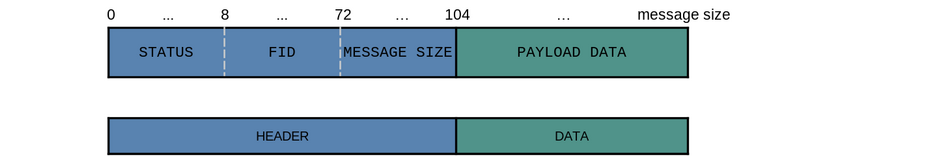
\includegraphics[width=\textwidth]{images/contributions/old-buffer-format.png}
\caption{Legacy buffer format with a 13-byte header. The numbers shown on top are bits}
\label{fig:old-buffer-format}
\end{figure}

\begin{figure}[htbp]
\centering
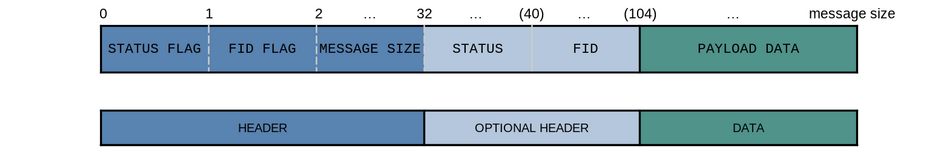
\includegraphics[width=\textwidth]{images/contributions/new-buffer-format.png}
\caption{Revised buffer format, reducing header overhead. The numbers shown on top are bits.}
\label{fig:new-buffer-format}
\end{figure}

This optimization works because data in the same \texttt{block} is guaranteed to have the same \acs{FID}.
Supposing messages of 20 bytes --- by being conservative in the estimate --- the first header will contain all the optional fields, meaning that the first message will be $13 + 20 = 33$ bytes. The next headers are guaranteed to have the same \acs{FID}, so they will be $4 + 20 = 24$ bytes each. A block will thus contain 42 messages --- $33 + (24 \times 41) = 1017$ bytes --- while before a block could contain 31 messages --- $31 \times 33 = 1023$ bytes. In a conservative estimate, with the new formatting a block can contain 30\% more messages.